% !TEX root =./main.tex

\section{Block 9: Contrast/Brightness - Chen \& Stentiford}

Contrast enhancement is a critical image processing technique used to improve the visibility and
distinction of objects within an image by adjust the intensity levels of its pixels. Objects of
interest often lie within certain ranges of gray levels, which requires contrast enhancement to
highlight these important features.


\subsection{Implementation}

To implement contrast enhancement, we utilized the window/level algorithm, as seen in Figure 1.
The algorithm takes each pixel value and determines whether to supress or enhance the pixel's
brightness with threshold values.

\begin{figure}[H]
    \centering
    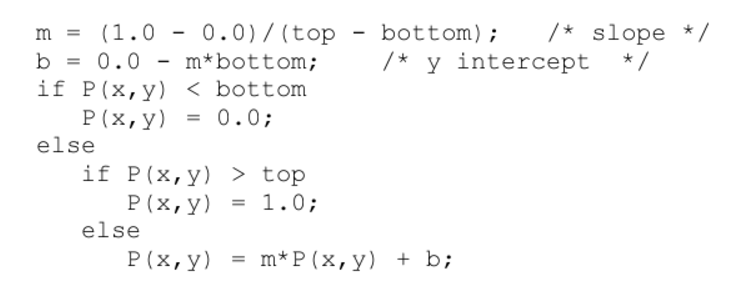
\includegraphics[width=0.5\linewidth]{figures/windowlevelalgorithm.png}
    \caption{Window/Level Algorithm}
    \label{fig:window/levelalgorithm}
\end{figure}

The contrast stage is difficult to optimize because the necessity of if-else statements precludes 
vectorization. To make the costly operation run as quickly as possible, we took the route of 
writing a native library for MATLAB in C (see contrastFix.c) to perform the operation. Not only 
are for loops written in C more performant compared to their MATLAB counterparts, C also allows 
for lower-level manipulation of data structures. In particular, 2D matrices in MATLAB require 
two index values (row and column) to access, meaning to iterate through each member of the matrix 
requires nested for loops, with the outer loop iterating through each row and the inner loop 
iterating through each member of each row. Internally, MATLAB stores all matrices as normal, 1D 
arrays (along with some metadata). As such, using C, we can iterate through each member of the matrix 
by simply looping through a normal array of numbers, meaning we only have to use one loop instead 
of a nested pair. Furthermore, C also allows specifying that certain variables should be stored in 
registers instead of memory, allowing for more efficient access of variables oft-needed for computation. 
Additionally, at the compile stage, some optimization parameters were passed to the compiler so that 
the resulting library was built with compiler code optimization, link-time optimization (where 
unnecessary function calls are bypassed), and forced usage of modern SSE (Streaming Single-Input-
Multiple-Data Extensions) instructions, which on current x86 CPUs, are more efficient than the 
standard x87 Floating Point instructions. Together, these elements ensure that the contrast stage 
ran as efficiently as possible.